\section{Теоретические основы}

Метрическое пространство~---~это пара $ \left( S, d \right) $,
состоящая из множества $S$ и метрики $d \; : \; S \times S \rightarrow \mathbb{R}$,
то есть для любых $x, y, z \in S$ выполняется
\begin{enumerate}
  \item $d \left( x, y \right) \geq 0$;
  \item $d \left( x, y \right) = 0 \Leftrightarrow x = y$~---~аксиома тождества;
  \item $d \left( x, y \right) = d \left( y, x \right) $~---~аксиома симметрии;
  \item $d \left( x, z \right) \leq d \left( x, y \right) + d \left( y, z \right) $ ---
  неравенство треугольника.
\end{enumerate}

Метрическое пространство $ \left( S, d \right) $ называется сепарабельным,
если существует не более чем счётное множества $ \Gamma \subset S \, : $
\begin{equation*}
  \forall x \in S \qquad
  \forall \varepsilon > 0 \qquad
  \exists y \in \Gamma\, : \qquad
  d \left( x, y \right) < \varepsilon.
\end{equation*}

Метрическое пространство $ \left( S, d \right) $ --- полное,
если в нём любая фундаментальная последовательность сходится.

Примером полного сепарабельного метрического пространства есть $ \mathbb{R}^n$
с евклидовым расстоянием.

\section{Расстояние Хаусдорфа}

Расстояние Хаусдорфа определяется на множестве
всех непустых замкнутых подмножеств пространства $ \mathbb{R}^n$.

Пусть $E$ и $F$~---~непустые замкнутые подмножества $ \mathbb{R}^n$.
Расстояние Хаусдорфа между $E$ и $F$ определяется как
\begin{equation}\label{eq:hausdorff:distance}
  H \left( E, F \right) =
  \inf \left\{ \varepsilon > 0 \; | \; E \subset F + \varepsilon, \, F = E + \varepsilon \right\},
\end{equation}
где $E + \varepsilon $~---~объединение замкнутых шаров
с центром в точке $x$ радиуса $ \varepsilon $
\begin{equation*}
  E + \varepsilon =
  \bigcup \limits_{x \in E} \left\{ \overline{B}_{ \varepsilon } \left( x \right) \right\}.
\end{equation*}

Докажем асиомы метрики, чтобы проверить, что расстояние Хаусдорфа $H \left( E, F \right) $,
заданое формулой \ref{eq:hausdorff:distance}~---~
это действительно расстояние между двумя замкнутыми множествами в $ \mathbb{R}^n$.

\begin{enumerate}
  \item $H \left( E, F \right) \geq 0$.
  Это следует из определения \ref{eq:hausdorff:distance},
  так как точная нижняя грань величины $ \varepsilon > 0$ неотрицательна.
  \item $H \left( E, F \right) = 0$ тогда и только тогда, когда $E = F$.
  Если $E = F$, то $E \subset F$ и $F \subset E$, то есть $H \left( E, F \right) = \varepsilon = 0$.
  С другой стороны, если $H \left( E, F \right) = 0$, то $ \varepsilon = 0$,
  то есть опять $E \subset F$ и $F \subset E$.
  Получаем, что $E = F$.
  \item $H \left( E, F \right) \leq H \left( E, F \right) + H \left( F, G \right) $
  для любых замкнутых множеств $E, F, G$ из $ \mathbb{R}^n$.
  Запишем правую часть по определению \ref{eq:hausdorff:distance}
  \begin{gather*}
    H \left( E, F \right) + H \left( F, G \right) = \\
    = inf \left\{
      \varepsilon_1 > 0 \; \middle| \; E + \varepsilon_1 \subset F, \, F + \varepsilon_1 \subset E
    \right\} + \\
    + inf \left\{
      \varepsilon_2 > 0 \; \middle| \; F + \varepsilon_2 \subset G, \, G + \varepsilon_2 \subset F
    \right\}.
  \end{gather*}
  Сумма инфимумов равна инфимуму суммы.
  Объединяя два множества, получаем
  \begin{equation*}
    E + \varepsilon_1 \subset F \subset F + \varepsilon_2 \subset G, \,
    G + \varepsilon_2 \subset F \subset F + \varepsilon_1 \subset E.
  \end{equation*}
  Собирая первые и последние части выражений, видим,
  что $E + \varepsilon \subset G$ и $G + \varepsilon \subset E$, а это левая часть неравенства.
\end{enumerate}

\subsection{Пример}

Найдём расстояние Хаусдорфа между двумя эллипсами \ref{fig:hausdorff:example} \cite{crownover}
\begin{gather*}
  E \, : \, \frac{x^2}{4} + 4y^2 = 1, \, \\
  F \, : \, 4 \left( x - 2 \right)^2 + \frac{y^2}{4} = 1.
\end{gather*}

\begin{figure}
  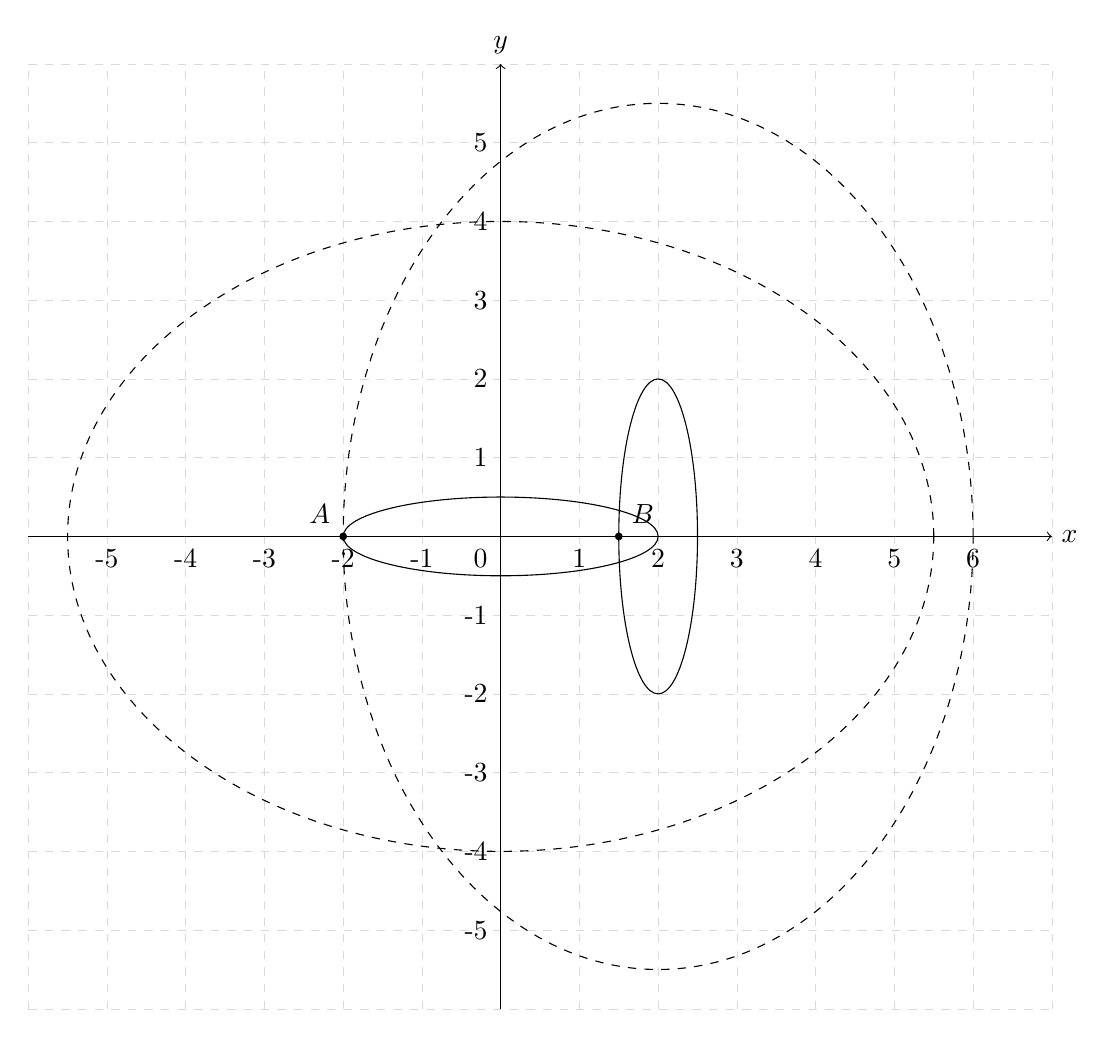
\begin{tikzpicture}
    \draw[help lines, color=gray!30, dashed] (-6,-6) grid (7,6);
    \draw[->] (-6,0)--(7,0) node[right]{$x$};
    \draw[->] (0,-6)--(0,6) node[above]{$y$};
    \node[inner sep=1pt,label=below left:{0}] at (0,0) {};
    \foreach \i in {-5,...,-1,1,2,3,4,5,6}
    {
      \node[inner sep=1pt,label=below:{\i}] at (\i,0) {};
    }
    \foreach \i in {-5,...,-1,1,2,3,4,5}
    {
      \node[inner sep=1pt,label=left:{\i}] at (0,\i) {};
    }
    \draw (0,0) ellipse (2 and 0.5);
    \draw (2,0) ellipse (0.5 and 2);
    \draw[dashed] (0,0) ellipse (5.5 and 4);
    \draw[dashed] (2,0) ellipse (4 and 5.5);
    \node[circle,inner sep=1pt,fill=black,label=above left:{$A$}] at (-2,0) {};
    \node[circle,inner sep=1pt,fill=black,label=above right:{$B$}] at (1.5,0) {};
  \end{tikzpicture}
  \caption{Эллипсы, между которыми ищем расстояние Хаусдорфа}
  \label{fig:hausdorff:example}
\end{figure}

Пунктиром нарисованы эллипсы $E + \varepsilon $ и $F + \varepsilon $ такие,
чтобы выполнялось \ref{eq:hausdorff:distance}.
Таким образом $ \varepsilon $ в данном случае~---~это расстояние между точками $A$ и $B$,
которое равно $ \varepsilon = 1.5 - \left( -2 \right) = 3.5$.
Поэтому $H \left( E, D \right) = 3.5$.

\section{Случайные величины}

Имеем вероятностное пространство $ \left( \Omega, \mathcal{F}, \mathbb{P} \right) $,
где $ \Omega = \mathbb{R}^n, \, \mathcal{F} = \mathcal{B} \left( \mathbb{R}^n \right) $~---~
борелевская $ \sigma$-алгебра на $ \mathbb{R}^n, \, \mathbb{P}$~---~
вероятностная мера на $ \mathcal{F}$.

Есть два определения случайной величины:
\begin{enumerate}
  \item функция $ \xi \, : \, \Omega \to \mathbb{R}$ называется случайной величиной, если
  \begin{equation*}
    \forall \Delta \in \mathcal{B} \left( \mathbb{R} \right) \, : \qquad
    \xi^{-1} \left( \Delta \right) =
    \left\{ \omega \; \middle| \; \xi \left( \omega \right) \in \Delta \right\} \in \mathcal{F};
  \end{equation*}
  \item функция $ \xi \, : \, \Omega \to \mathbb{R}$ называется случайной величиной, если
  \begin{equation*}
    \forall c \in \mathbb{R} \, : \qquad
    \left\{ \omega \; \middle| \; \xi \left( \omega \right) \leq c \right\} =
    \xi^{-1} \left( \left( -\infty, c \right] \right) \in \mathcal{F}.
  \end{equation*}
\end{enumerate}

Хотим проверить,
является ли расстояние Хаусдорфа
\begin{equation*}
  \gamma =
  H \left( AE + \vec{b} + \vec{ \xi }, F \right) =
  H \left( \xi \left( E \right), F \right)
\end{equation*}
случайной величиной, где $ \xi $~---~
случайное отображение из $ \mathbb{R}^n$ в $ \mathbb{R}^n$.

По определению \ref{eq:hausdorff:distance}
$ \gamma =
  \inf \limits_n \left\{
    \varepsilon_n \; \middle| \;
    \xi \left( E \right) + \varepsilon_n \subset F, \,
    F + \varepsilon_n \subset \xi \left( E \right) \right\} $.

Чтобы это проверить, нужно выяснить, является ли случайной величиной число $ \varepsilon_n > 0$.
Если получится, то
\begin{equation*}
  \forall c \in \mathbb{R}: \qquad
  \left\{ \omega \; \middle| \; \inf \limits_n \varepsilon_n \left( \omega \right) \leq c \right\} =
  \bigcup \limits_{n = 1}^{ \infty }
    \left\{ \omega \; \middle| \; \varepsilon_n \left( \omega \right) \leq c \right\}.
\end{equation*}
Каждое множество, которые стоит под знаком объединения, по определению,
принадлежит $ \sigma $-алгебре $ \mathcal{F}$,
и их счётное объединение принадлежит $ \sigma $-алгебре $ \mathcal{F}$,
так как она замкнута относительно счётной операции объединения.
